\section{Einführung}
\subsection{Erzwungene Schwingung}
Wenn auf ein Schwingsystem von außen ein periodisches Drehmoment $M_0cos(\omega t)$ wirkt, ändert sich die Bewegungsgleichung des freien gedämpften Pendels (vgl. Protokoll zu M1) zu
\begin{equation}
J\ddot{\varphi}+r\dot{\varphi}+D\varphi=M_0cos(\omega t).
\end{equation}
Diese Formel lautet in der Normalform
\begin{equation}
\ddot{\varphi}+2p\dot{\varphi}+\omega_0^2\varphi= \mu cos(\omega t) \text{   mit   } \mu=M_0/J.
\end{equation}
Nach dem Ende des Einschwingvorgangs, beim Einschalten der Anregung entstandene freie Schwingungen sind abgeklungen, ist der sogenannte stationäre Zustand erreicht, die äußere Energiezufuhr ist genau gleich dem Energieverlust durch die Dämpfung. Im stationären Zustand gilt
\begin{equation}
\varphi (t)= \varphi_0cos(\omega t-\alpha)
\end{equation}
mit der Amplitude
\begin{equation}
\varphi_0=\frac{\mu}{\sqrt{(\omega^2-\omega_0^2)^2+4p^2\omega^2}}
\label{eq:amplitude}
\end{equation}
und der Phase
\begin{equation}
tan \alpha = \frac{-2p\omega}{\omega^2-\omega_0^2}.
\label{eq:phase}
\end{equation}
Beim sogenannten Resonanzfall mit $\omega=\sqrt{\omega_0^2-2p^2}$ ist die Amplitude maximal und es kann für dämpfungsfreie Systeme($p\rightarrow 0 \Rightarrow \omega = \omega_0$), zur Resonanzkatastrophe kommen, sprich die Amplitude schaukelt sich bis ins unendliche hoch.
\subsection{Drehpendel nach Pohl}
Beim dem Drehpendel nach Pohl handelt es sich um eine Schwingscheibe, die von einem Exzenters angeregt und mit Hilfe einer Wirbelstrombremse wiederum gedämpft werden kann. Da der Exzenter an der Spiralfeder greift und die Wirbelstrombremse ausschaltbar ist, können mit dem Drehpendel von Pohl sämtliche Schwingungsarten, freie, gedämpfte und erzwungene Schwingung, nachvollzogen werden.
\begin{figure}[h]
  \centering
  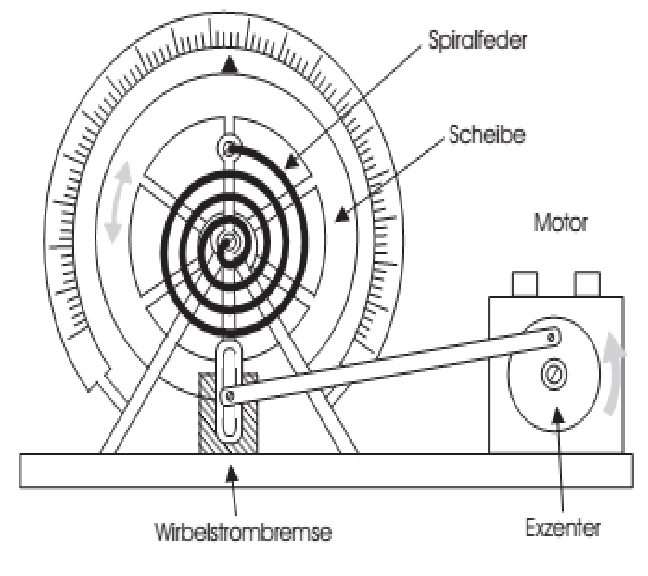
\includegraphics[width=0.5\textwidth]{Drehpendelpohl}
  \caption{Drehpendel nach Pohl \footcite{anleitung-ws2014}}
  \label{fig:drehpendel}
\end{figure}
\section{Versuche}
\subsection{Aufgabe 2}
Schon vor Durchführung der Messungen fällt auf, dass auch bei ausgeschalteter Wirbelstrombremse eine Dämpfung vorliegt. Diese ist augenscheinlich groß genug, als dass die Bezeichnung ``näherungsweise ungedämpft'' aus der Versuchsanleitung fraglich ist.

Die Eigenfrequenz $\omega_0$ des Drehpendels wurde zunächst mit einer Stoppuhr über 10 Schwingungsperioden bestimmt. Die Messwerte lauten:
\begin{table}[H]
  \centering
  \begin{tabular}{c c c c} \toprule
    Messung & 1 & 2 & 3 \\ \midrule
    $10T$ & \SI{18.25(50)}{s} & \SI{18.21(50)}{s} & \SI{18.25(50)}{s} \\ \bottomrule
  \end{tabular}
  \caption{Schwingungsdauer mit Stoppuhr}
  \label{tab:stoppuhr}
\end{table}

Aus dem Mittelwert $10T=\SI{18.24(29)}{s}$ wurde die Eingenfrequenz berechnet:
\begin{equation}
  \omega_{0,\text{Uhr}}=\frac{2\pi}{T}=\SI{3.445(55)}{Hz}
  \label{eq:omega0uhr}
\end{equation}

Anschließend wurde die Messung über den Computer wiederholt. Im Diagramm ist die Auslenkung $\omega$ gegen die Zeit $t$ aufgetragen. Es ist zu beachten, dass es sich um die Auslenkung des an den Computer angeschlossenen Rades handelt, welches wiederum über einen Faden mit dem Drehpendel gekoppelt ist. Die genaue Auslenkung des Drehpendels ist aber nicht relevant zur Bestimmung der Eigenfrequenz.
\begin{figure}[H]
  \centering
  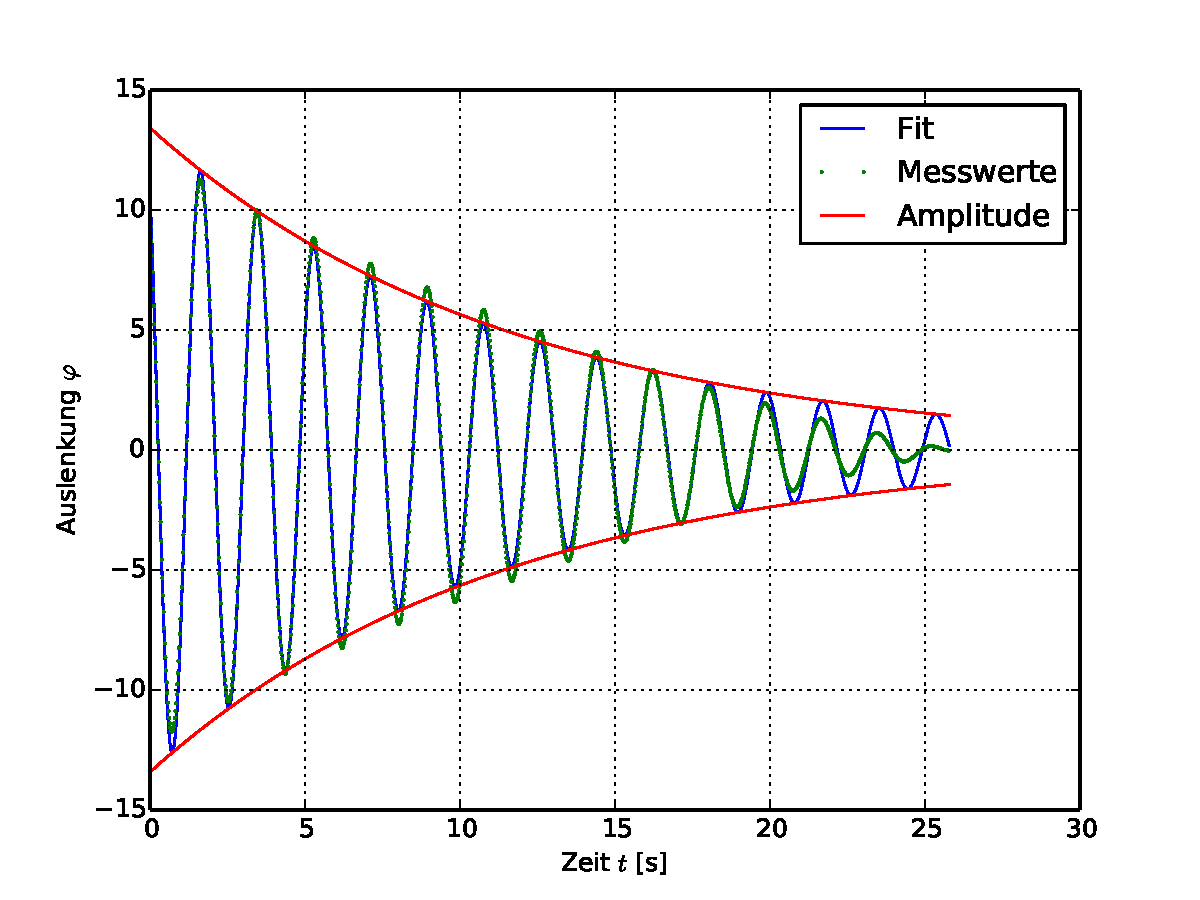
\includegraphics[scale=0.8]{computerdaten/Auswertung/2b)ungedaempft}
  \caption{Eigenfrequenz aus Computermessung}
  \label{fig:omega0pc}
\end{figure}
Wieder fällt die Dämpfung auf, die das Pendel nach \SI{25}{s} zum Stillstand bringt. Der Fit sowie die Einhüllende wurde mithilfe von SciPy nach dem Levenberg-Marquardt Algorithmus bestimmt. Die Ausgabe ist:
\begin{equation}
  \omega_{0.Fit}=\SI{3.443(1)}{Hz}
  \label{eq:omega0pc}
\end{equation}
Die relative Abweichung zwischen den beiden Werten beträgt $\frac{\omega_{0.Fit}-\omega_{0.Fit}}{\omega_{0.Fit}}\approx \SI{0.06}{\percent}$.
\subsection{Aufgabe 3}
Nun wurde die Wirbelstrombremse nacheinander mit $\SI{0.25(1)}{A}$,  $\SI{0.5(1)}{A}$ und $\SI{1.0(1)}{A}$ angesteuert und das Drehpendel mit der Hand ausgelenkt. In den Diagrammen ist wieder die Auslenkung gegen die Zeit aufgetragen.
\begin{figure}[H]
  \centering
  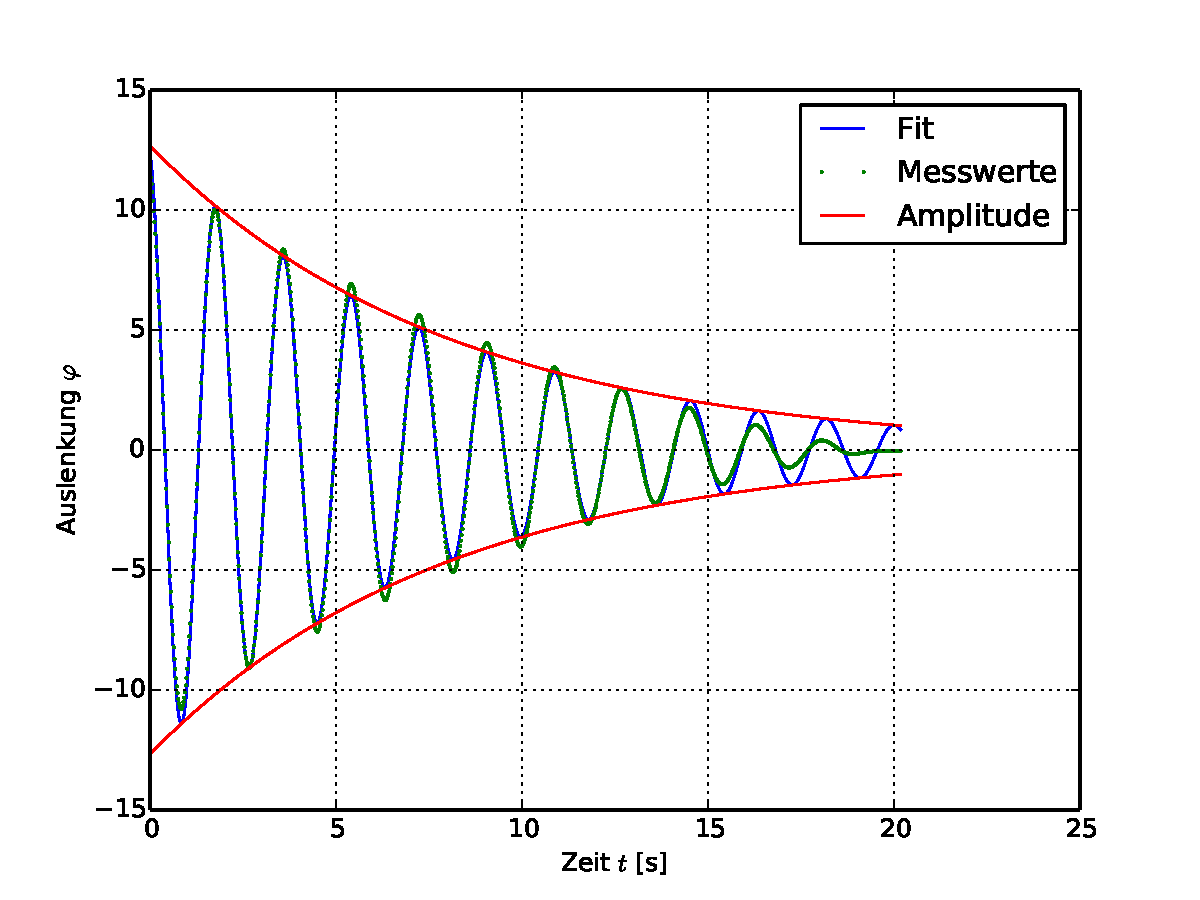
\includegraphics[height=9cm, width=15cm]{computerdaten/Auswertung/3)250mA}
  \caption{Messung für Dämpfung \SI{0.25}{A}}
  \label{fig:3_250}
\end{figure}
\begin{figure}[H]
  \centering
  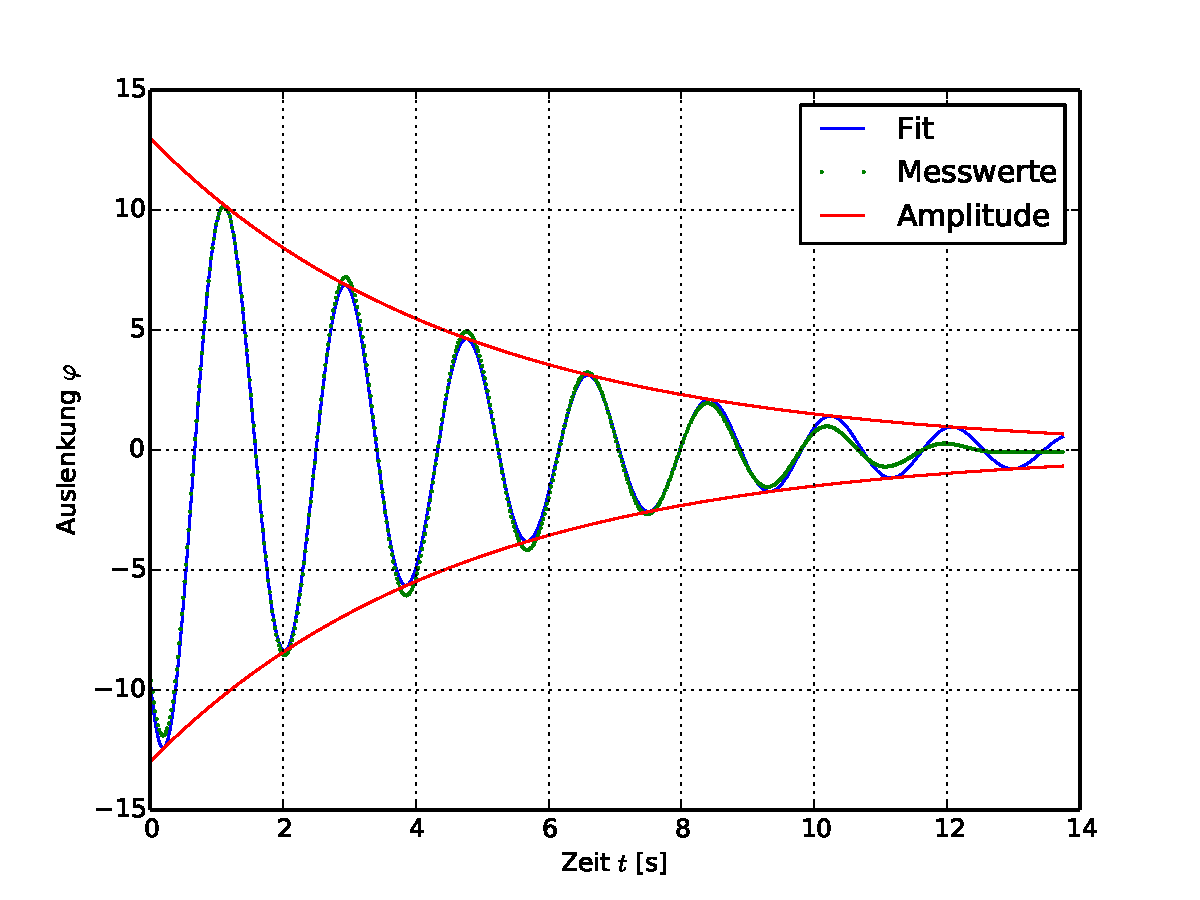
\includegraphics[height=9cm, width=15cm]{computerdaten/Auswertung/3)500mA}
  \caption{Messung für Dämpfung \SI{0.25}{A}}
  \label{fig:3_500}
\end{figure}
\begin{figure}[H]
  \centering
  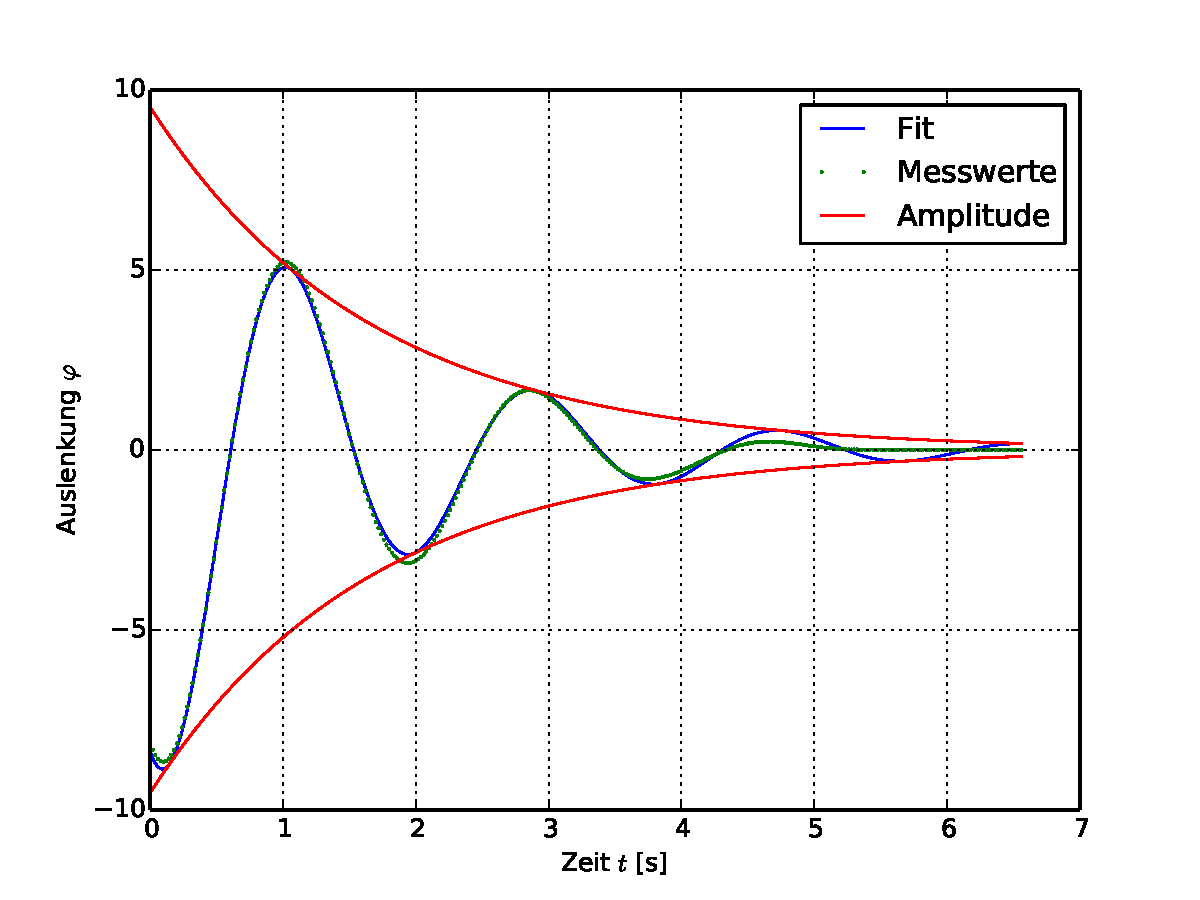
\includegraphics[height=9cm, width=15cm]{computerdaten/Auswertung/3)1000mA}
  \caption{Messung für Dämpfung \SI{1.0}{A}}
  \label{fig:3_1000}
\end{figure}
Aus dem Fit und der Einhüllenden wurde jeweils die Eigenfrequenz $\bar{\omega}$ und die Dämpfung $\rho$ bestimmt:
\begin{table}[H]
  \centering
  \begin{tabular}{c c c c} \toprule
    Dämpfungsstrom [\si{A}] & \num{.25} & \num{.5} & \num{1.0} \\ \midrule
    $\bar{\omega}$ [\si{Hz}] & \num{3.4437(1)} & \num{3.4401(1)} & \num{3.3987(1)} \\
    $\rho$ [\si{Hz}] & \num{.125202(1)} & \num{0.215880(2)} & \num{.603888(18)} \\ \bottomrule
  \end{tabular}
  \caption{Eigenfrequenz und Dämpfung}
  \label{tab:omegarho}
\end{table}
Es ist deutlich zu erkennen, dass $\rho$ mit größerem Dämpfungsstrom zunimmt.
\subsection{Aufgabe 4 und 5}
In diesem Versuch untersuchen wir die Abhängigkeit der Amplitude von Dämpfung und Anregefrequenz. Das Drehpendel mit der aus den vorherigen Versuchen bekannten Eigenschwingfrequenz wird mit Hilfe des Exzenters zu einer erzwungenen Schwingung angeregt. Nach dem Einschwingen wird jeweils die Amplitude gemessen, und gegen die Anregefrequenz aufgetragen. Dies führt man für zwei verschiedene Dämpfungen durch. Hierzu wird die Wirbelstrombremse mit verschiedenen Stromstärken betrieben.\\
Zur Auswertung muss die Drehfrequenz des Motors bekannt sein. Diese ist in dem von uns betrachteten Spannungsbereich linear zur Motorspannung. Daher bestimmen wir zunächst den Zusammenhang zwischen Spannung und Freqeunz aus Messungen bei verschiedenen Spannungen.
\begin{figure}[h]
	\centering
	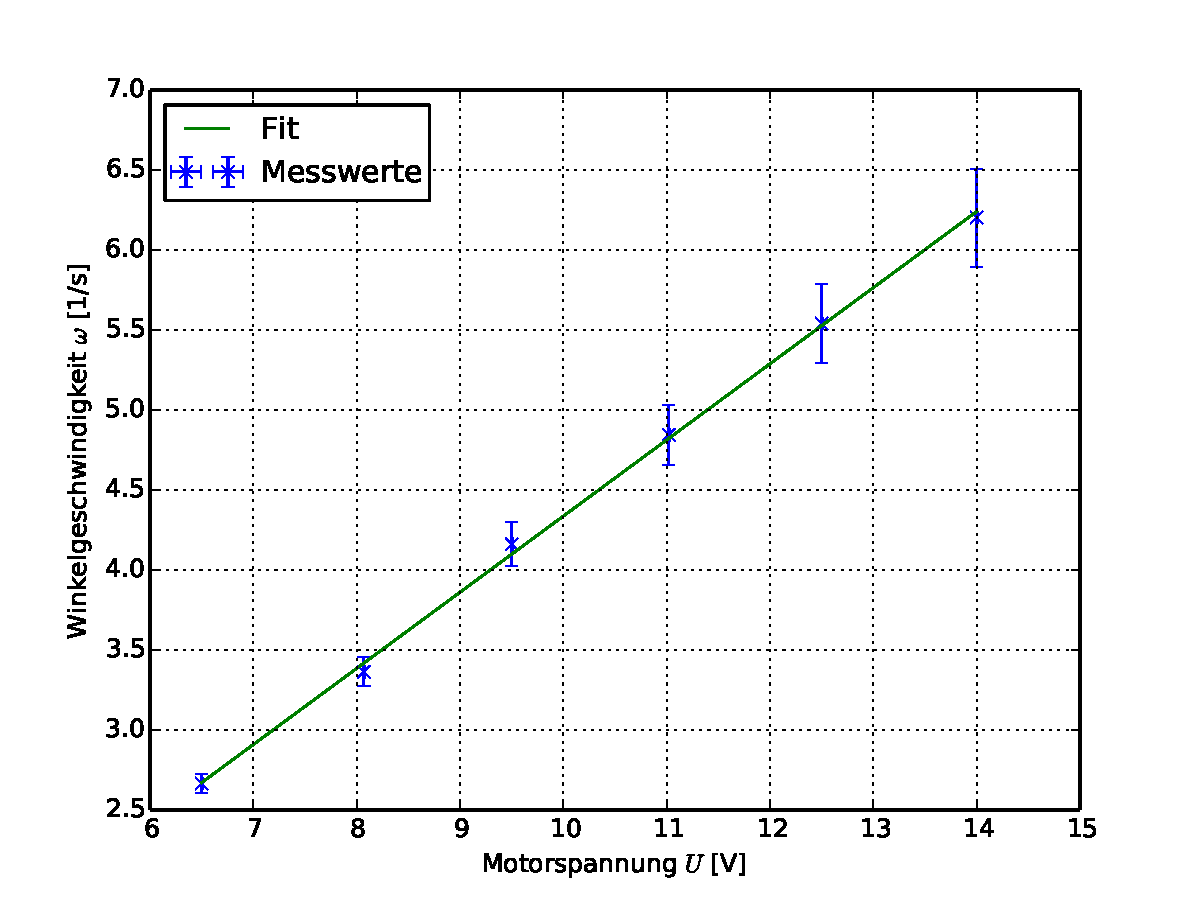
\includegraphics[width=\linewidth]{diagramme/eichkurve.pdf}
	\caption[Eichkurve]{Gemessene Spannungen gegen Winkelgeschwindigkeit aufgetragen}
	\label{fig:Eichkurve}
\end{figure}\\
Aus dem Fit der Messwerte erhält man unter Minimierung der Abstandsquadrate die Steigung $ (0{,}4759 \pm 0{,}0275)~\si{\per\second\per\volt} $ und den Achsenabschnitt $ (-0{,}4220 \pm 0{,}0804) \si{\per\second} $. Somit kann man durch 
\begin{equation*}
	\omega = \SI{0.4759}{\per\second\per\volt} U - \SI{-0.4220}{\per\second} \qquad \text{(+berücksichtigung der Fehler)}
\end{equation*}
$ U $ in $ \omega $ umrechnen. Trägt man $ \omega $ gegen die Amplitude $ \varphi $ auf, so ergibt sich Abbildung \ref{fig:Erzwungen}.
\begin{figure}[h]
	\centering
	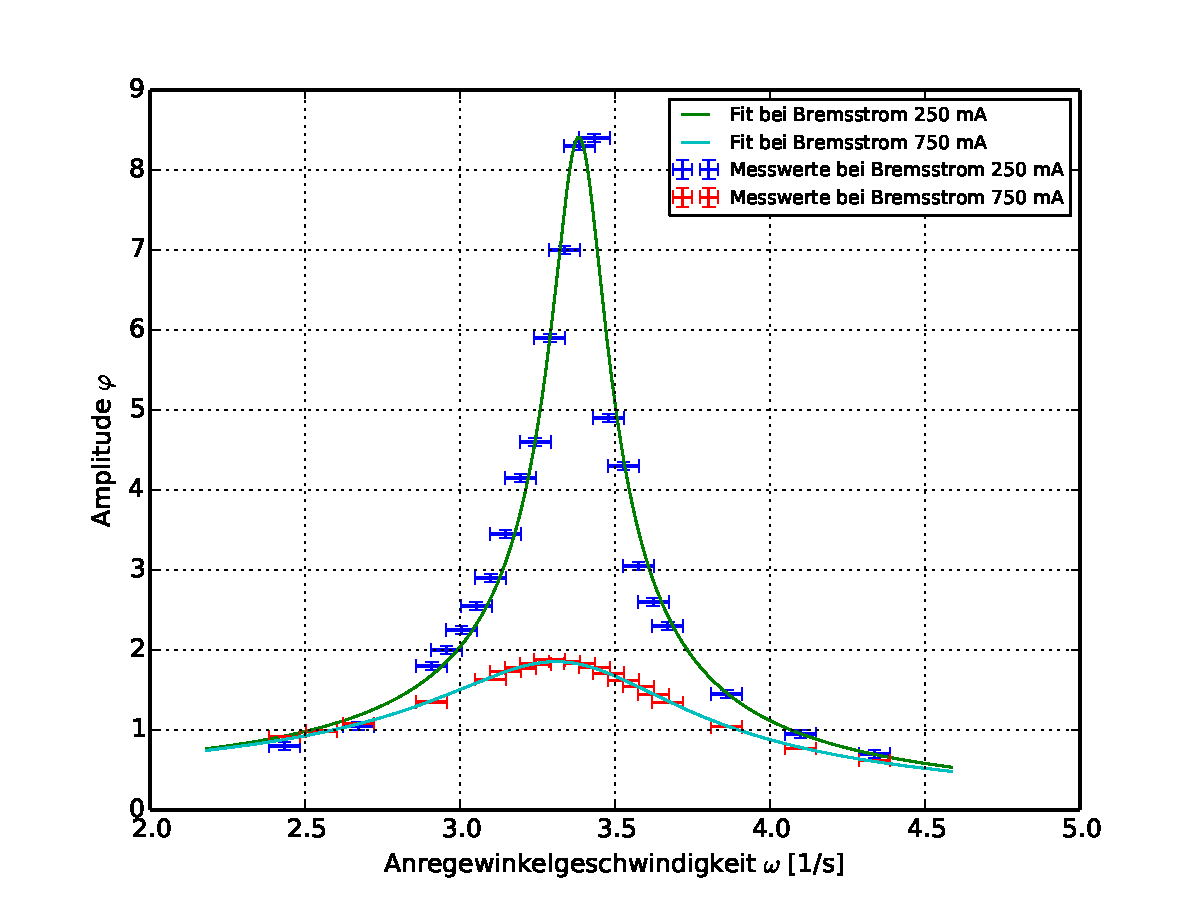
\includegraphics[width=\linewidth]{diagramme/5).pdf}
	\caption[Amplitudenfunktion]{Amplitude gegen Anregefrequenz aufgetragen}
	\label{fig:Erzwungen}
\end{figure}\\
Der Fit wurde mit der aus der Theorie bekannten Funktion für die Amplitude einer erzwungenen Schwingung erstellt. Der Fit unter Minimierung der Fehlerquadrate liefert als einen der Parameter die Dämpfung. Somit ist die Dämpfung jeweils:\\
\begin{tabular}{r@{: }l}
$ \SI{250}{\milli\ampere} $ & $ (0{,}090 \pm 0{,}010)~\si{\per\second} $ \\
$ \SI{750}{\milli\ampere} $ & $ (0{,}407 \pm 0{,}010)~\si{\per\second} $
\end{tabular}
\subsection{Aufgabe 6 / 7}
Der Dämpfungsstrom wurde auf \SI{0.25}{mA} eingestellt und die Phasenbeziehung zwischen Anregung und Drehpendel sowie die Amplitude bei drei verschiedenen Anregungsfrequenzen beobachtet:
\begin{enumerate}
  \item Bei einer Anregungsfrequenz \textit{geringer} als die Resonanzfrequenz sind die Anregung und das Drehpendel fast in Phase. Allerdings hinkt das Drehpendel der Anregung leicht hinterher.
Die Amplitude ist genauso groß wie die Amplitude der Anregung.
  \item Bei der \textit{Resonanzfrequenz} beträgt die Phasenverzögerung ungefähr $-\pi/2$, d.h. das Drehpendel erreicht ein Auslenkungsmaximum, wenn die Anregung gerade die Ruheposition durchläuft.
    Die Amplitude wird hier maximal.
  \item Bei sehr \textit{hohen} Frequenzen schwingen Anregung und Pendel fast genau gegensinnig (die Phasenverzögerung beträgt $-\pi$). 
    Die Amplitude wird sehr gering.
\end{enumerate}

Dieselben Beobachtungen wurden beim Fadenpendel gemacht.
\subsection{Aufgabe 8}
Es wurde ein kleines Gewicht neben dem Pfeil am Drehpendel angebracht und die Resonanzkurve ohne Dämpfung zweimal durchgefahren:
\begin{enumerate}
  \item von niedriger zu hoher Frequenz 
  \item von hoher zu niedriger Frequenz
\end{enumerate}
Dabei wurde beobachtet, dass die Amplitude beim 1. Durchlauf ein höheres Maximum erreicht, bevor sie dann rapide abfällt.
Im 2. Durchlauf blieb die Amplitude niedriger und fiel langsamer ab.
\section{Diskussion}
Bei den näherungsweise ungedämpften Schwingung wurde in beiden Messmethoden eine Eigenfrequenz $\omega_0$ mit einer Abweichung von nur $\SI{.06}{\percent}$ ermittelt. Dies ist erstaunlich, da die Messung mit Stoppuhr einem hohen Fehler durch die Reaktionszeit des Stoppenden ausgesetzt ist. Die Computermessung hat den Wert aber mit deutlich geringerem Fehler bestätigt. 
Physikalisch ist zu sagen, dass die Eigenfrequenz tatsächlich nach Abklingen der Einschwingvorgänge konstant beleibt. Dies ist aus \cref{fig:omega0pc} besonders gut ersichtlich. Allerdings ist zweifelhaft, ob wirklich die Eigenfrequenz ohne Dämpfung $\omega_0$ gemessen wurde, da im selben Diagramm eine recht starke Dämpfung ersichtlich ist. Der wahre Wert für $\omega_0$ liegt also etwas höher.\\

Bei den gedämpften Schwingungen (Aufgabe 3) wurden physikalisch zwei Beobachtungen gemacht:
\begin{enumerate}
  \item Bei höherem Dämpfungsstrom steigt wie erwartet der aus der Einhüllenden bestimmte Dämpfungsfaktor $\rho$. Die Amplitude nimmt also bei höheren Dämpfungen deutlich schneller ab, was auch in \crefrange{fig:3_250}{fig:3_1000} zu erkennen ist
  \item Die Eigenfrequenz $\bar{\omega}$ sinkt mit steigender Dämpfung, was aus dem theoretischen Zusammenhang $\bar{\omega}=\sqrt{\omega_0^2-\rho^2}$ erwartet ist. 
\end{enumerate}
Da wie oben angesprochen das System auch ohne Wirbelstrombremse schon gedämpft war, ist ein Anteil des Dämpfungsfaktors $\rho$ auf diese Dämpfung zurückzuführen.\\

Zu Aufgabe 4 / 5:
Die theoretisch ermittelten Zusammenhänge decken sich gut mit unseren Beobachtungen. Insbesondere an Abbildung \ref{fig:Erzwungen} ist zu sehen, dass sich eine Ausgleichskurve entsprechend der Theorie fitten lässt, die ziemlich genau durch die Messwerte geht. Jedoch war wie auch bei vorherigen Versuchen eine die größte Quelle der Unsicherheit die Zeitnahme mit der Stoppuhr. Zudem stellten wir beim Erstellen der Eichkurve fest, dass sich der Motor schon knapp unterhalb der betrachteten Spannungen nicht mehr linear bezüglich der Frequenzen verhält. Damit erklärt sich unter anderem auch, dass die Ausgleichsgerade keine Ursprungsgerade ist.\\

In Bezug auf die Frequenzabhängigkeit von Amplitude und Phase wurden durch die Beobachtungen die Zusammenhänge aus \cref{eq:amplitude,eq:phase} bestätigt. Dies betrifft das Maximum der Amplitude im Resonanzfall sowie den Phasenverlauf von 0 bei kleinen Frequenzen zu $-\pi$ bei sehr großen. \\

Nach Anbringen eines Gewichtes wurde festgestellt, dass das System sich unterschiedlich verhält, je nachdem ob man das Frequenzspektrum von unten oder von oben durchfährt. Dies deutet auf nichtlineares bzw. chaotisches Verhalten hin.
\notecite{anleitung-ws2014}
